\documentclass[conference]{IEEEtran}
\IEEEoverridecommandlockouts
% The preceding line is only needed to identify funding in the first footnote. If that is unneeded, please comment it out.

\usepackage{booktabs}
\usepackage{amsmath,amssymb,amsfonts, mathabx}
% \usepackage[backend=biber,style=alphabetic,sorting=ynt]{biblatex}
% \addbibresource{sample.bib} %Import the bibliography file
\usepackage{enumitem}
\usepackage{algorithmic}
\usepackage{physics}
\usepackage{graphicx}
\usepackage{textcomp}
\usepackage[colorlinks=true, allcolors=black]{hyperref}
\usepackage{xcolor}
\usepackage{multirow}
\def\BibTeX{{\rm B\kern-.05em{\sc i\kern-.025em b}\kern-.08em
    T\kern-.1667em\lower.7ex\hbox{E}\kern-.125emX}}
\begin{document}
\title{Optimal drone overtaking using Model Predictive Control\\}
\author{\IEEEauthorblockN{Akash John Subash}
\IEEEauthorblockA{\textit{M.Sc. Embedded Systems Engineering} \\
\textit{Albert-Ludwig's University Freiburg}\\
MatrNr. 5253501}
}

\maketitle

\begin{abstract}
This project report describes the formulation of an optimal overtake aerial maneuver computed in real time using Model Predictive Control (MPC). Limited implementation details in python with CasADi and the crazyFlie 2.1 drone are also mentioned.

\end{abstract}

\section{Introduction}\label{Introduction}
The Crazyflie 2.1 quadcopter is a versatile open source flying development platform with expansion decks that make it a good candidate for university projects. The optimal controls computed offboard using MPC are fed to the crazyFlie, with the intention to overtake a second quadcopter (henceforth referred to as obstacle).

The structure of the report is as follows: Section \hyperref[Section2]{II} describes the model and the dynamics of the crazyFlie 2.1 quadcopter using Ordinary Differential Equations (ODE). Section \hyperref[Section3]{III} shows the optimal control problem, it's non-linear program and section \hyperref[Section4]{IV}, \hyperref[Section5]{V} detail the control topologies in open and closed-loop. Section \hyperref[Section6]{VI} presents the results 
of simulation and flight tests. Finally, section \hyperref[Section7]{VII}, \hyperref[Section8]{VIII} acknowledges the resources which were referred to, and the guidance received during the course of the project.

\section{System Modelling}\label{Section2}
\begin{figure}[htbp]
	\centerline{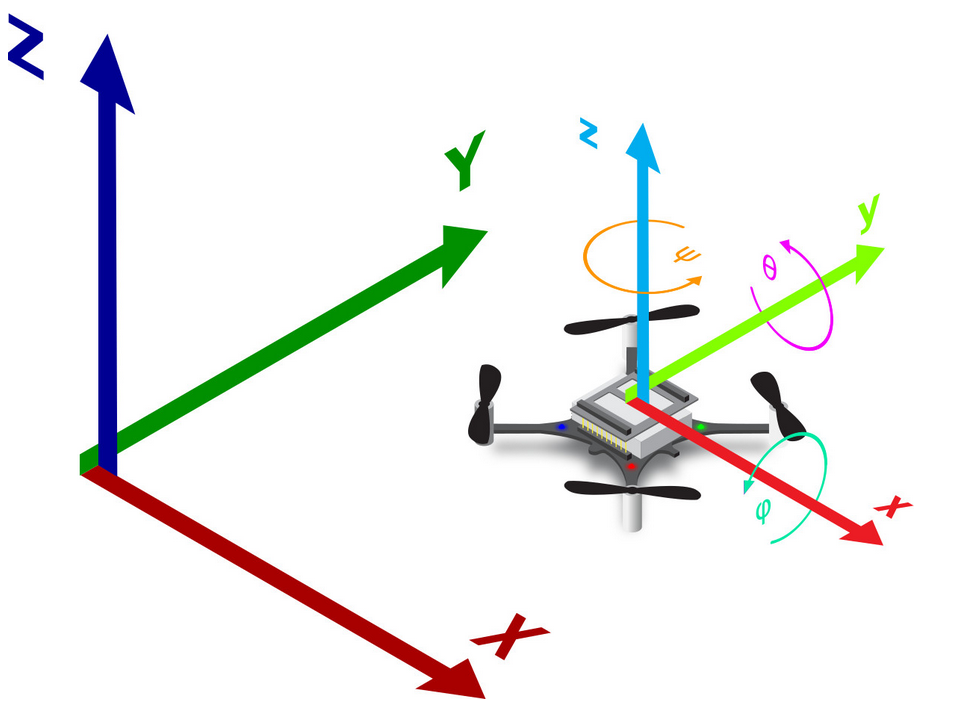
\includegraphics[scale = 0.4]{figures/ordinate.png} }
	\caption{Reference coordinate system [1]}
	\label{Fig1}
\end{figure}
As depicted in \hyperref[Fig1]{Fig. 1}, a body frame located at the centre of mass of the quadcopter aligned with the East-North-Up inertial frame is used here, with $\varphi$, $\theta$, $\psi$ representing roll, pitch and yaw in the Euler notation respectively.

\subsection{Physical model of the drone}
The state $\zeta$ $\in$ $\mathbb{R}$ $\mathrm{^{13}}$ of the drone can be described by position $p$ = ($x$, $y$, $z$)$\mathrm{^{T}}$, attitude in quaternion notation $q$ = ($q_{w}$, $q_{x}$, $q_{y}$, $q_{z}$)$\mathrm{^{T}}$, linear velocities $v$ = ($v_x$, $v_y$, $v_z$)$\mathrm{^{T}}$, and angular velocities $\omega$ = ($\omega_x$, $\omega_y$, $\omega_z$)$\mathrm{^{T}}$. It's non-linear dynamics are given by the ODE, which are adapted from \cite{carlos_efficient_2020} and \cite{Luis_2016}, making changes to describe attitude in quaternion instead of Euler notation.\\

\begin{align*}
\dot{\zeta} &= \begin{bmatrix}
	\dot{p} \\
	\dot{q}\\
	\dot{v}\\
	\dot{\omega}
\end{bmatrix} =
\begin{bmatrix}
    Sv \\
    \frac{1}{2}q\times \omega\\
    \frac{1}{m}F - S\mathrm{^{T}}g1_z - \omega \times v\\ 
    J\mathrm{^{-1}}(M - \omega \times J \omega)\\
\end{bmatrix}\\
\end{align*}
 
The model parameters are described in \hyperref[table1]{Table I}. The quaternion rotation matrix $S$ $\in$ $\mathbb{R}$ $\mathrm{^{3\times3}}$, external force matrix $F$ $\in$ $\mathbb{R}$ $\mathrm{^{3\times1}}$, external momentum matrix $M$ $\in$ $\mathbb{R}$ $\mathrm{^{3\times1}}$, and inertial matrix $J$ $\in$ $\mathbb{R}$ $\mathrm{^{3\times3}}$ are described below.\\
\hfill\break

\begin{align*}
	S &=
	\begin{bmatrix}
		2(q_w \mathrm{^{2}} + q_x \mathrm{^{2}}) - 1 & 
		2(q_x q_y - q_w q_z) & 
		2(q_w q_y + q_y q_z) \\
		2(q_w q_z + q_x q_y) &
		2(q_w \mathrm{^{2}} + q_y \mathrm{^{2}}) - 1 & 
		2(q_y q_z - q_w q_x) \\
		2(q_x q_z - q_w q_y) & 
		2(q_w q_x + q_y q_z) & 
		2(q_w \mathrm{^{2}} + q_z \mathrm{^{2}}) - 1\\
	\end{bmatrix}
\end{align*}
\hfill\break

\begin{align*}
	F &=
	\begin{bmatrix}
		0 \\
		0 \\
		C_t(\Omega_1\mathrm{^{2}} + \Omega_2\mathrm{^{2}} + \Omega_3\mathrm{^{2}} + \Omega_4\mathrm{^{2}})\\ 
	\end{bmatrix}
\end{align*}
\hfill\break

\begin{align*}
	J &=   
	\begin{bmatrix}
		I_{xx} & 0 & 0\\
		0 & I_{yy} & 0\\
		0 & 0 & I_{zz}\\ 
	\end{bmatrix}
\end{align*}
\hfill\break

\begin{align*}
	M &=
	\begin{bmatrix}
		\frac{1}{\sqrt{2}}\,dC_t(-\Omega_1\mathrm{^{2}} - \Omega_2\mathrm{^{2}} + \Omega_3\mathrm{^{2}} + \Omega_4\mathrm{^{2}})\\
		\frac{1}{\sqrt{2}}\,dC_t(-\Omega_1\mathrm{^{2}} + \Omega_2\mathrm{^{2}} + \Omega_3\mathrm{^{2}} - \Omega_4\mathrm{^{2}})\\
		C_d(-\Omega_1\mathrm{^{2}} + \Omega_2\mathrm{^{2}} - \Omega_3\mathrm{^{2}} + \Omega_4\mathrm{^{2}})\\
	\end{bmatrix}
\end{align*}
Given the possibility to individually change the angular velocities of the propellers, the control vector is defined as: \\                          
$u$ := ($\Omega_{1}$, $\Omega_{2}$, $\Omega_{3}$, $\Omega_{4}$)$\mathrm{^{T}}$ $\in$ $\mathbb{R}\mathrm{^{4}}$

\begin{table}[htbp]
	\small
	\begin{center}
		\begin{tabular}{lccccl}\toprule
			\textbf{Description} &  \textbf{Symbol}\\
			\midrule
            $\mathrm{Mass\,of\,the\,drone} \,m$ & $\mathrm{31 \cdot 10^{-3}\,\mathrm{kg}}$  \\
			$\mathrm{Drone\,arm\,length} \,d$ & $46 \cdot \mathrm{10^{-3}}\,\mathrm{m}$ \\
			$\mathrm{Inertial\,moment} \,I_{xx}$ & $1.395 \cdot\,\mathrm{10^{-5}} \mathrm{kg\,m^2}$ \\
            $\mathrm{Inertial\,moment} \,I_{yy}$ & $1.395 \cdot\,\mathrm{10^{-5}} \mathrm{kg\,m^2}$ \\
            $\mathrm{Inertial\,moment} \,I_{zz}$ & $2.173 \cdot\,\mathrm{10^{-5}} \mathrm{kg\,m^2}$ \\
            $\mathrm{Coefficient\,of\,drag} \,C_d$ & $\mathrm{7.93 \cdot 10^{-12}}\,\mathrm{N\,RPM^{-2}}$ \\
			$\mathrm{Coefficient\,of\,thrust} \,C_t$ & $\mathrm{3.25 \cdot 10^{-10}}\,\mathrm{N\,RPM^{-2}}$ \\
			$\mathrm{Gravitational\,acceleration} \,g$ & $\mathrm{9.81 \cdot\,m\,s^{-2}}$ \\
			\bottomrule
		\end{tabular}
	\end{center}
	\caption{Parameters of the model}
	\label{table1}
\end{table}

\begin{figure*}[htbp]
	\centerline{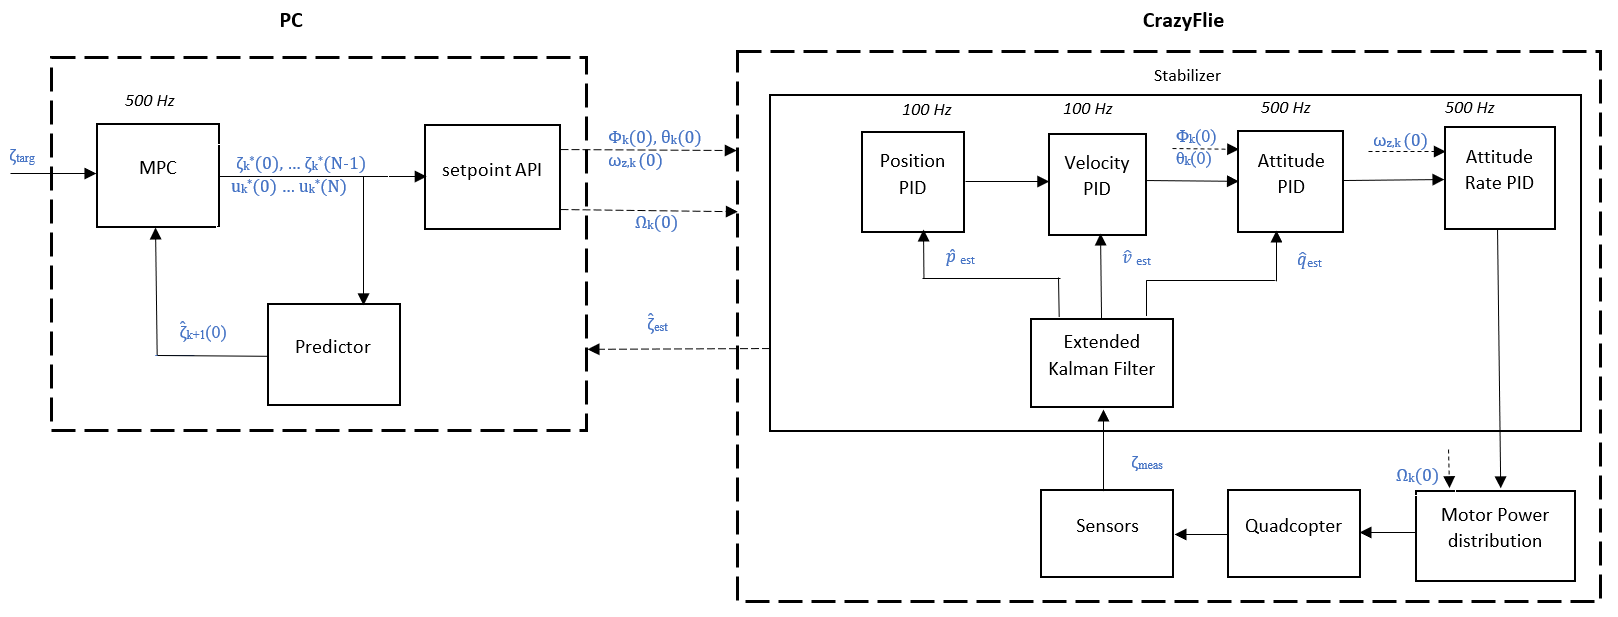
\includegraphics[scale = 0.6]{figures/Screenshot_OL.png} }
	\caption{Open loop control architecture }
	\label{Fig2}
\end{figure*}

\subsection{State Predictor}

A state predictor based on the explicit Runge-Kutta integrator (RK4) was implemented to approximate the state evolution. Starting from the current measured state, forward iterations of the system dynamics are performed with an appropriate time step ($\tau_{s}$) chosen to minimize the approximation error in the state evolution.

To solve the control problem in real time, it's important to consider the radio communication latency between the off-board processor running the MPC algorithm and the quadcopter. This impacts the delay in receiving measurements ($\tau_{r}$) from the quadcopter and sending control commands to it ($\tau_{t}$). Additionally, with an associated computational delay ($\tau_{c}$) for calculating optimal solutions, the round trip delay of $\tau_{trr}$ = $\tau_r$ + $\tau_t$ + $\tau_c$ is defined. While $\tau_{r}$, $\tau_{t}$ are considered constants, the impact of variation of $\tau_{c}$ is discussed in the following chapters.

\section{Problem Formulation}\label{Section3}

In this section, the discretized Optimal Control Problem (OCP) and its constrained Non-Linear Program (NLP) are defined using direct multiple shooting \cite{bock_multiple_1984} to discretize the underlying continuous time OCP.

\subsection{Optimal Control Problem}

The initial state is defined as the quadcopter hovering at a height $z$ = 0.5 m, and the goal is to reach a specified target state avoiding another quadcopter along the way, at position  $p_\mathrm{b}$ = ($x_\mathrm{b}$, $y_\mathrm{b}$, $z_\mathrm{b}$)$\mathrm{^{T}}$

The discretized cost function is defined as :
\begin{align}
	& L\left(\zeta_k, U_k\right) = \lVert \zeta_k - \zeta_{\mathrm{trg}} \rVert^2_Q + \lVert u_k - u_{\mathrm{hov}} \rVert^2_R
\end{align}

The OCP is then formulated as :
\begin{align}
	&\min_{u_0,\zeta_0,..,u_{N-1},\zeta_N} \quad \sum_{k = 0}^{N-1} L(\zeta_k, u_k) \\
	\text{s.t} \quad 
	& \zeta_0 - \bar{\zeta_0} \hspace{0.42in} = 0\\
    & \zeta_k - F(\zeta_k, u_k) = 0, \hspace{0.1in}\quad\qquad k = 0,..,N-1 \\
    & 3\,\mathrm{d} \hspace{0.1in} \le \lVert p_k - p_{\mathrm{b}} \rVert \le  \infty, \qquad  k = 0,..,N-1 \\
	& \zeta_{\mathrm{min}} \le \hspace{0.22in} \zeta_k \hspace{0.25in} \le \zeta_{\mathrm{max}}, \quad k = 0,..,N-1 \\
    & 0 \hspace{0.2in} \le \hspace{0.23in} u_k \hspace{0.22in} \le U_{\mathrm{max}} \quad k = 0,..,N-1
\end{align}

\begin{flushleft}
$\bar{\zeta_0}$ \hspace{0.18in}= $(0, 0, 0.5, 1, 0, 0, 0, 0, 0, 0, 0, 0, 0)^T$\\
$\zeta_{\mathrm{trg}}$ \hspace{0.08in}= $( 1, 1, 1, 1, 0, 0, 0, 0, 0, 0, 0, 0, 0)^T$\\
$\zeta_{\mathrm{max}}$ \hspace{0.03in}= $(1.5,1.5,1.5,\infty,\infty,\infty,\infty,0.25,0.25,0.25,\frac{\pi}{4},\frac{\pi}{4},\frac{\pi}{4})^T$\\
$\zeta_{\mathrm{min}}$ \hspace{0.05in}= -$\zeta_{\mathrm{max}}$\\
$U_{\mathrm{max}}$ = $(22000, 22000, 22000, 22000)^T$\\
$p_\mathrm{b}$ \hspace{0.18in}= $(0.5, 0.5, 0.5)^T$\\
\end{flushleft}

Where $\zeta := (\zeta_0, .., \zeta_N)^T$, and $u := (u_0, .., u_{N-1})^T$ denote the state and control trajectories of the discrete time system. The discretized dynamics are given by the RK-4 integrator $F :$ $\mathbb{R}^{n_{\zeta}} \cdot \mathbb{R}^{n_{u}} \rightarrow \mathbb{R}^{n_{\zeta}}$ (Referred to as predictor in Figure 2). The horizon length and the estimated state of the system at the current time instant $k$ are denoted by $N$, and $\zeta_k$ respectively.

 $Q$ $\in$ $\mathbb{R}^{n_{\zeta} \cdot n_{\zeta}}$ and $R$ $\in$ $\mathbb{R}^{n_{u} \cdot n_{u}}$ are positive definite weighting matrices, tuned experimentally for the specific flight trajectory to be executed.
\begin{flushleft}
\begin{small}
$Q$ = diag\begin{footnotesize}$(120, 100, 100, 10^{-3}, 10^{-3},10^{-3},1, 1, 1, 1, 10^{-5}, 10^{-5}, 10^{-5})$\\
\end{footnotesize}
$R$ = diag\begin{footnotesize}$(8 \cdot 10^{-1}, 8\cdot 10^{-1}, 8\cdot 10^{-1}, 8\cdot 10^{-1})$\\
\end{footnotesize}
\end{small}
\end{flushleft}

\section{Open-loop Control }\label{Section4}
The open-loop control of the drone without the obstacle to be avoided was implemented with a horizon of $N = 10$ in python using the CasADi \cite{andersson_casadi_2019} framework with IPOPT \cite{wachter_implementation_2006} as the interior point NLP solver. Using the next state predicted by the RK4 integrator from the current state and controls, the MPC computes the optimal solution iteratively. The optimal open-loop controls for each time could only be fed with minimal delay to the quadcopter, by solving the problem offline. 


However, the large error propagation causing the quadcopter to quickly veer off the estimated trajectory, warrants the closed loop problem, and argues against placing the obstacle in the quadcopter's flight path in open loop.
The appropriate set-point command API provided by the open source crazy-flie libraries allowed to communicate the controls as a set of roll, pitch, yaw rate, and thrust. 

\section{Closed-loop Control }\label{Section5}
Using the same solver framework, the estimated state from the Extended Kalman filter onboard the Crazyflie sampled at 50 Hz, was fed back to the MPC algorithm for closed loop control. To minimize radio communication latency arising from the reception of multiple data frames, it was read in a compressed format via a single frame from the stabilizer module onboard and decoded on the PC. The sampling rate was determined by the lower bound on the achievable computation time of the solver. Using MPC to control the system, an instance of (2) is solved iteratively at each sampling time point, with the current value of the state estimate $\zeta_k$. 

The closed loop architecture differs from Figure 2, only in the feedback path, where the predictor computes $\hat{\zeta}_{k+1}$ from $\hat{\zeta}_{\mathrm{est}}$ instead of $\zeta^*_{k}$.
In closed loop, adding the obstacle to be avoided necessitated increasing the horizon to $N$ = 20 for a smooth control, and state trajectory which led to a large increase in computation time ($\tau_c$). In order to use the state estimated in the feedback path, online iterations of the MPC was mandatory. As a consequence, the 500 Hz MPC computation rate could no longer be maintained and fell significantly to 50 Hz.

\section{Closed-loop Control Results}\label{Section6}

The most important factor to consider while moving from simulations to hardware flights were delays. The choice of 
$\tau_s$ was made to ensure the quadcopter's state, control trajectory evolution were plausible, while trying to maintain a minimal $\tau_c$. A value of $\tau_s$ = 20 ms was found to provide a good trade-off between the two. 
The round trip delay $\tau_{trr}$ was found to be dominated by $\tau_{c}$ which is dependant on the choice of the solver framework, and the integration step ($\tau_s$) of the non-linear system dynamics, among other factors.

\begin{figure}[htbp]
	\centerline{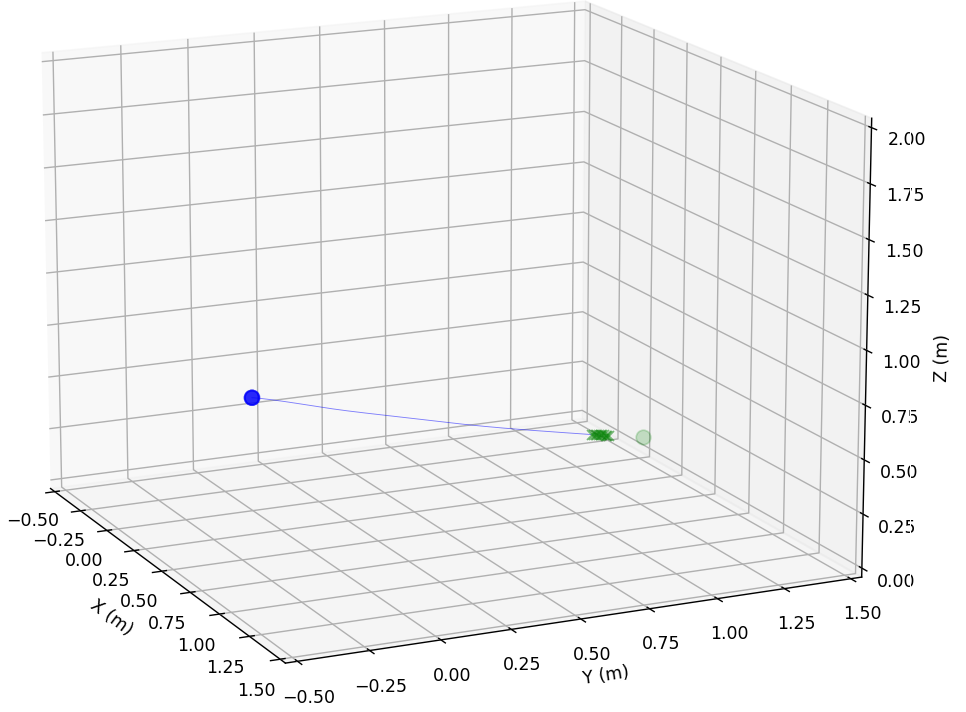
\includegraphics[scale = 0.4]{figures/Screenshot_OL_ST.png} }
	\caption{Open loop trajectory without obstacle for $N$ = 10, $\tau_s$ = 20ms}
	\label{Fig3}
\end{figure}

\begin{figure}[htbp]
	\centerline{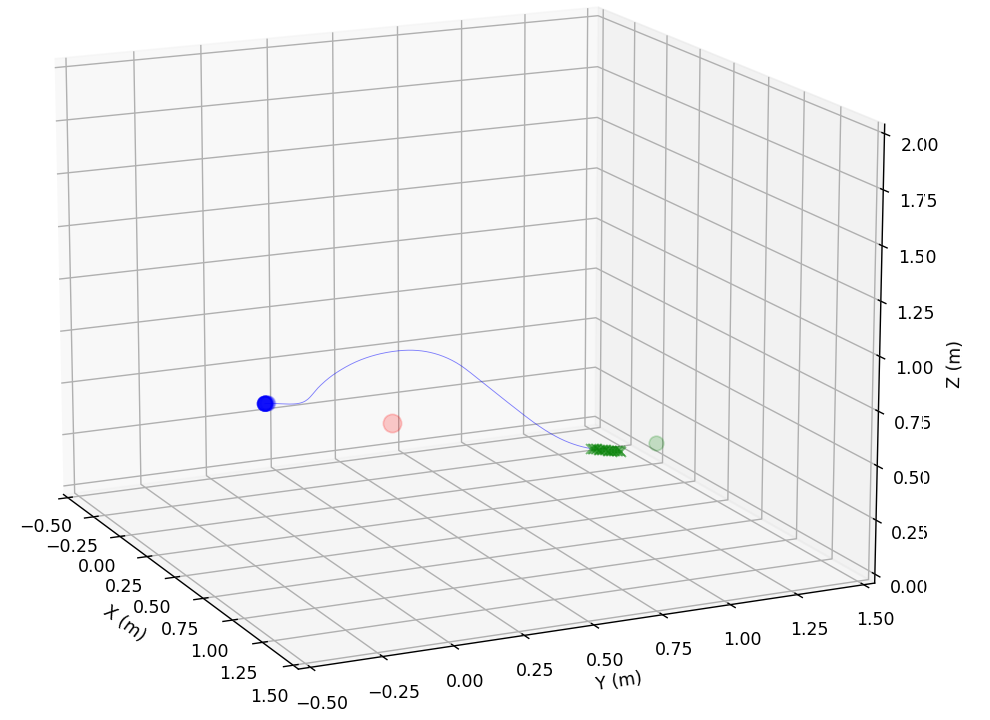
\includegraphics[scale = 0.4]{figures/Screenshot_OLwO_ST.png} }
	\caption{Open loop trajectory with obstacle for $N$ = 20, $\tau_s$ = 20ms}
	\label{Fig4}
\end{figure} 


In the open, and closed loop flights without the obstacle, $\tau_{trr}$ was sufficiently small to observe stable flights. In closed loop, with the obstacle and $N$ = 10, the quadcopter's attempt at aggressively avoiding the obstacle would cause the state estimated by the online stabilizer module to have large errors, arguing for a larger horizon length $N$. Choosing $N$ = 20 provided a smooth control trajectories in simulation, but at the expense of a large $\tau_{c}$ which was no longer sufficient to control the quadcopter in a stable flight path. 

\begin{figure*}[t!]
	\centerline{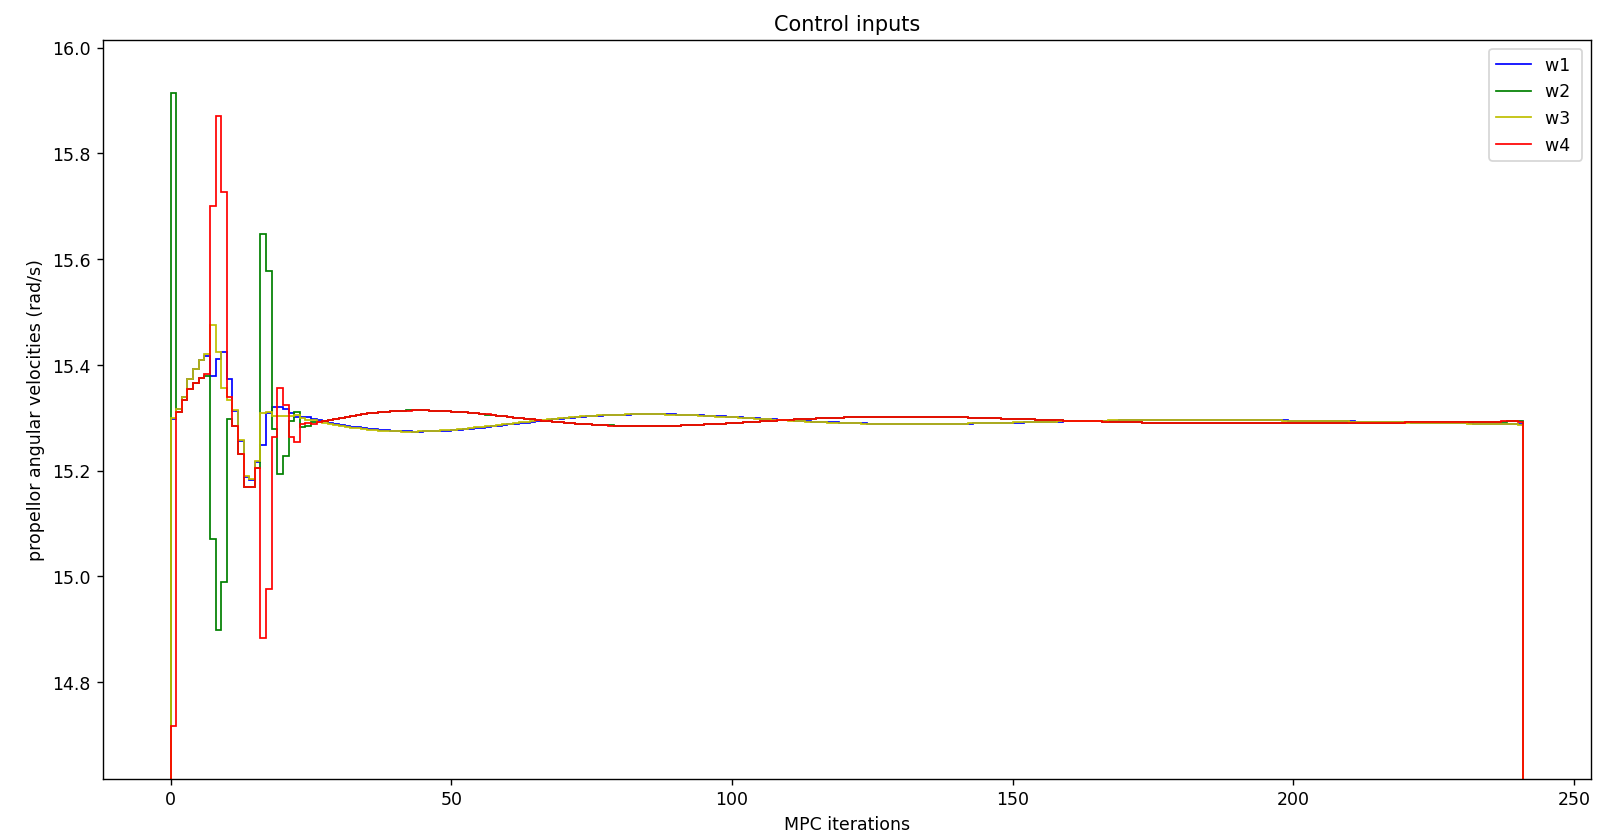
\includegraphics[scale = 0.45]{figures/Screenshot_OL_U.png} }
	\caption{Open loop controls without obstacle for $N$ = 10, $\tau_s$ = 20ms, $\tau_c$ = 40ms}
	\label{Fig5}
\end{figure*}

The average iteration time achieved in closed-loop for computation without obstacle avoidance was $\tau_{c}$ = 40 ms, and $\tau_{c}$ = 100 ms with obstacle avoidance on an Intel i7-8750H processor @2.2Ghz running Windows. Future attempts could include reformulating the NLP as a sequential quadratic program (SQP) and using acados \cite{verschueren_acados_2020} with structure exploiting solvers to further reduce $\tau_c$ to achieve the overtake maneuver in real time.



\section{Acknowledgements}\label{Section7}
I would like to thank Mohammed Hababeh, Jakob Harzer, Andrea Ghezzi and Prof. Dr. Moritz Diehl for their supervision and guidance in this project.

\bibliographystyle{ieeetr}
\bibliography{./bibliography/sample.bib}
\end{document}